\documentclass{article}

\usepackage[spanish]{babel}
\usepackage[utf8]{inputenc}
\usepackage[T1]{fontenc}
\usepackage{graphicx}
\usepackage{hyperref}
\usepackage{courier}
\usepackage{listings}
\usepackage{xcolor}
\usepackage{blindtext}
\usepackage{scrextend}
\usepackage[document]{ragged2e}
\usepackage{multicol}
\usepackage{pgfgantt}
\usepackage{mathtools}
\usepackage{minted}
\usepackage{tikz}
\usepackage{longtable}
\usepackage{algorithm}
\usepackage[noend]{algpseudocode}
\usepackage{amsmath}
\usepackage{wrapfig,lipsum,booktabs}
\usepackage{fontspec}
 % % % % % % % %

\setmainfont{Calibri}

\hypersetup{
	colorlinks,
	linkcolor={blue!60!black},
	citecolor={blue!50!black},
	urlcolor={blue!80!black}
}

\usetikzlibrary{positioning,fit,calc}

\usemintedstyle{pastie}

\usepackage{array}
\newcolumntype{L}[1]{>{\raggedright\let\newline\\\arraybackslash\hspace{0pt}}m{#1}}
\newcolumntype{C}[1]{>{\centering\let\newline\\\arraybackslash\hspace{0pt}}m{#1}}
\newcolumntype{R}[1]{>{\raggedleft\let\newline\\\arraybackslash\hspace{0pt}}m{#1}}

\def\labelitemi{\textbf{--}}

\usepackage{anysize}
\marginsize{2.54cm}{2.54cm}{2.54cm}{2.54cm}

\usepackage{setspace}
%\onehalfspacing
\doublespacing

\makeatletter
\newcommand*{\MoveFitHeight}[1]{%
	\pgfmathsetlengthmacro\fit@inner@sep{%
		\pgfkeysvalueof{/pgf/inner xsep}%
	}%
	\pgfmathsetlengthmacro\fit@text@height{%
		\tikz@text@height
	}%
	\kern-\fit@inner@sep\relax
	\raisebox{\fit@text@height}[0pt][0pt]{#1}%
}
\makeatother

\newcommand{\bigO}[1]{$O({#1})$}

\setlength{\columnsep}{1cm}

%En caso de que LaTeX separe las palabras con - de manera incorrecta, usar
%\hyphenation{deci-sión,e-xa-men, otras palabras....}

\begin{document}
%--% Portada %------------------------------------------%
\centerline{Universidad de Carabobo}
\centerline{Facultad de Ciencia y Tecnologia}
\centerline{Sistemas Operativos}
\vspace{7cm}
\begin{centering}
	\hrule 	\vspace{0.4cm}
	{ \Huge \bfseries Segmentación y Paginación \\[0.4cm] }
	\hrule \vfill
\end{centering}
\vfill
\centerline{Victor Tortolero, 24.569.609}
\centerline{\today}
\newpage
%-------------------------------------------------------%

%-------------------------------------------------------%
{\centering \section*{Determinación del Tamaño de la página}}
El tamaño de una pagina es una potencia de $2$, que varia entre $512$ bytes y $1$ GB por pagina, dependiendo de la arquitectura del sistema. Se usan potencias de $2$ para el tamaño de pagina ya que la traducción se hace mas fácil.

A pesar de que el tamaño de pagina esta bastante relacionado con el hardware, el sistema operativo puede elegir cambiarlo. Por ejemplo, con páginas de 512 bytes, el sistema operativo puede considerar fácilmente los pares de páginas 0 y 1, 2 y 3, 4 y 5, y así en lo sucesivo, como páginas de 1 KB al asignar siempre dos marcos de página de 512 bytes consecutivos para ellas.

Si tenemos un tamaño de paginas muy grande ocurre fragmentación interna porque se esta desperdiciando espacio. Y en el caso de un tamaño de paginas muy pequeño implica que los programas necesitaran muchas paginas, y se perdería mucho tiempo transfiriendo paginas desde y hacia el disco.

Si el tamaño del espacio de direcciones lógicas es $2^m$, y el tamaño de pagina es $2^n$ byte, entonces los $m - n$ bits mas significativos de una dirección lógica indican el numero de pagina, y los $n$ bits menos significativos indican el desplazamiento de pagina.

\begin{figure}[H]
	\centering
	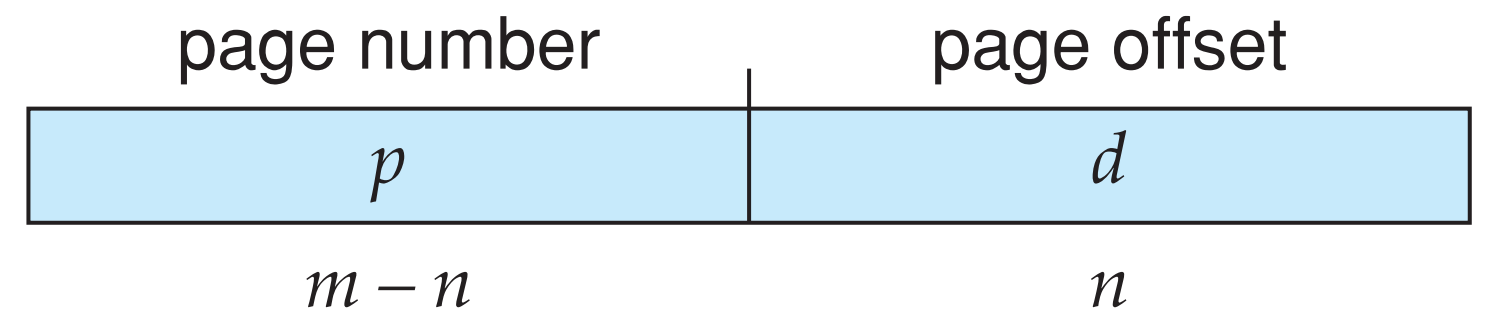
\includegraphics[scale=0.25]{img/direccion_logica.png}
	\caption{Dirección Lógica}
\end{figure}


%-------------------------------------------------------%
{\centering \section*{Tabla de páginas invertidas}}
En la tabla de paginas invertida, se tiene una entrada por cada pagina real (o marco) de memoria. Cada entrada consiste de una dirección virtual de la pagina guardada en esa dirección de memoria real, con información acerca del proceso al que pertenece la pagina.

Este esquema reduce la cantidad de memoria necesaria para guardar cada tabla de paginas, incrementa la cantidad de tiempo necesario para buscar en la tabla cuando se produce una referencia a una pagina.

En los sistemas que usan tablas de pagina invertidas, se tienen dificultades para implementar memoria compartida. La memoria compartida es usualmente implementada como varias direcciones virtuales (una por cada proceso compartiendo memoria) que corresponden a una dirección física. Este método es imposible realizarlo con la pagina de tablas invertida, porque solo hay una entrada de pagina virtual por cada pagina física. Para resolver esto, se puede permitir que la tabla de paginas sólo contenga una única correspondencia de una dirección virtual con la dirección física compartida, entonces las referencias a direcciones virtuales que no estén asociadas darán como resultado un fallo de pagina.

\begin{figure}[H]
	\centering
	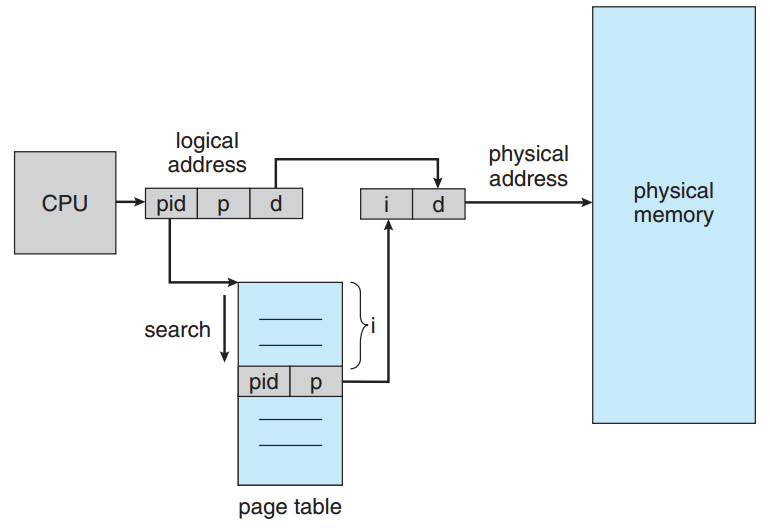
\includegraphics[scale=0.5]{img/pagina_invertida.png}
	\caption{Tabla de paginas invertida}
\end{figure}


%-------------------------------------------------------%
{\centering \section*{Tabla de páginas multinivel}}
Una solución para el gasto de memoria de la tabla de paginas, es paginar la tabla de paginas. Entonces tendríamos una tabla de paginas multinivel, o una jerarquía de tablas. Existe una única tabla de paginas de primer nivel. Cada entrada de esta tabla apunta a las tablas del segundo nivel. A su vez, las tablas de pagina de segundo nivel apuntan a las tablas de pagina de tercer nivel, y asi sucesivamente por cada nivel de la jerarquía. Las tablas de pagina del ultimo nivel apuntan directamente a marcos de pagina. Normalmente esta jerarquía esta limitada a dos o tres niveles. 

A la hora de traducir una dirección lógica, el número de pagina contenida en la misma se considera dividido en tantas partes como niveles existen.

La ventaja de este modelo es que si todas las entradas de una tabla de páginas de cualquier nivel están marcadas como inválidas, no es necesario almacenar esta tabla de páginas. Bastaría con marcar como inválida la entrada de la tabla de páginas de nivel superior que corresponde con esa tabla vacía, logrando reducir el gasto de memoria.

\begin{figure}[H]
	\centering
	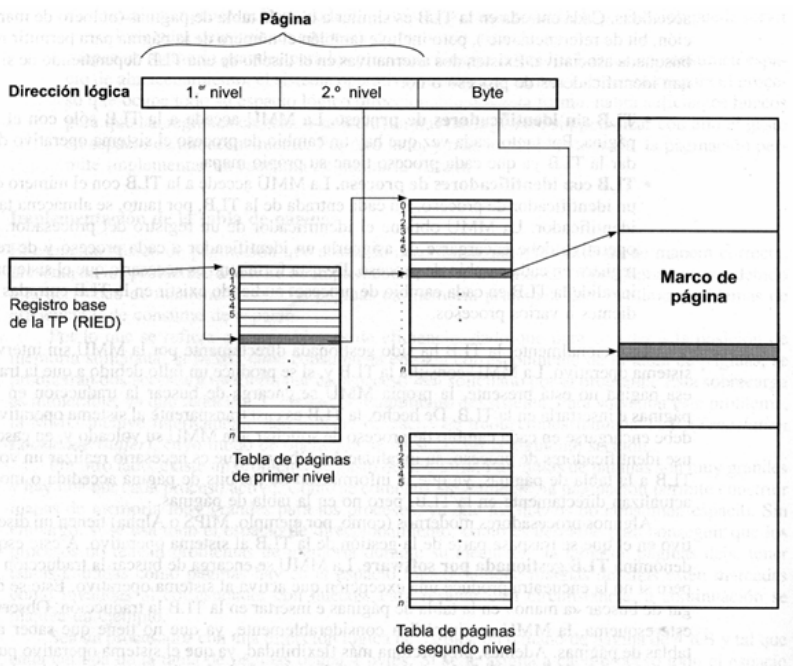
\includegraphics[scale=0.6]{img/paginacion_multi.png}
	\caption{Tabla de paginas multinivel con 2 niveles}
\end{figure}


%-------------------------------------------------------%
{\centering \section*{Protección de la memoria cuando se utiliza la paginación y la segmentación}}

\subsection*{Paginación}
La protección de memoria se logra con bits de protección asociados a cada marco. Estos bits normalmente se mantienen en la tabla de paginas.

Un bit podría indicar si una pagina es de lectura-escritura o solo lectura. Cuando se este calculando la dirección física, los bits de protección pueden ser revisados para verificar que no se hacen escrituras a una pagina de solo lectura. Esto puede extenderse para lograr un mayor nivel de protección, ya se a con hardware, o tener bits separados para cada tipo de acceso. Cualquier intento ilegal (por ejemplo, escritura en una pagina de solo lectura) causara un trap de hardware al sistema operativo.

Generalmente se asocia un bit adicional a cada entrada de la tabla de paginas, un bit válido-inválido. Cuando el bit esta en valido, la pagina asociada se encuentre en el espacio de direcciones lógicas del proceso y entonces es una pagina legal o valida. Si el bit esta en invalido, la pagina no se encuentre en el espacio de direcciones lógicas del proceso. Las direcciones ilegales se capturan utilizando este bit. El sistema operativo configura este bit para cada pagina para permitir o prohibir el acceso a dicha pagina.

\begin{figure}[H]
	\centering
	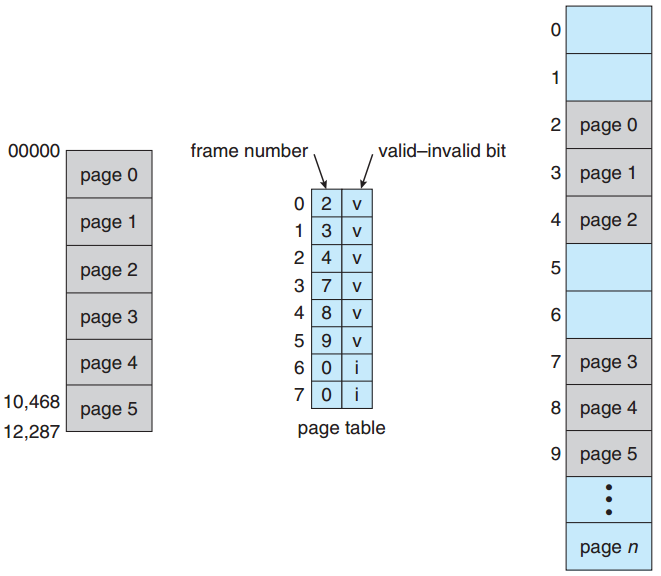
\includegraphics[scale=0.6]{img/paginacion_proteccion.png}
	\caption{Bit valido-invalido en una tabla de paginas}
\end{figure}

\subsection*{Segmentación}
La protección de memoria se logra con bits de protección asociados a cada marco. Estos bits normalmente se mantienen en la tabla de paginas.

Un bit podría indicar si una pagina es de lectura-escritura o solo lectura. Cuando se este calculando la dirección física, los bits de protección pueden ser revisados para verificar que no se hacen escrituras a una pagina de solo lectura. Esto puede extenderse para lograr un mayor nivel de protección, ya se a con hardware, o tener bits separados para cada tipo de acceso. Cualquier intento ilegal (por ejemplo, escritura en una pagina de solo lectura) causara un trap de hardware al sistema operativo.

Generalmente se asocia un bit adicional a cada entrada de la tabla de paginas, un bit válido-inválido. Cuando el bit esta en valido, la pagina asociada se encuentre en el espacio de direcciones lógicas del proceso y entonces es una pagina legal o valida. Si el bit esta en invalido, la pagina no se encuentre en el espacio de direcciones lógicas del proceso. Las direcciones ilegales se capturan utilizando este bit. El sistema operativo configura este bit para cada pagina para permitir o prohibir el acceso a dicha pagina.

\begin{figure}[H]
	\centering
	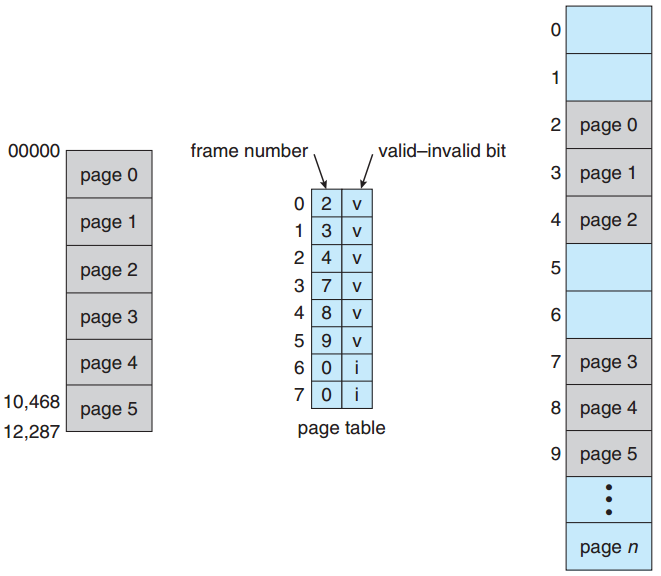
\includegraphics[scale=0.6]{img/paginacion_proteccion.png}
	\caption{Bit valido-invalido en una tabla de paginas}
\end{figure}


%-------------------------------------------------------%
{\centering \section*{Compartición de la memoria cuando se utiliza paginación o segmentación}}

\subsection*{Paginación}
Una ventaja de la paginación es la posibilidad de compartir código en común. 

\begin{figure}[H]
	\centering
	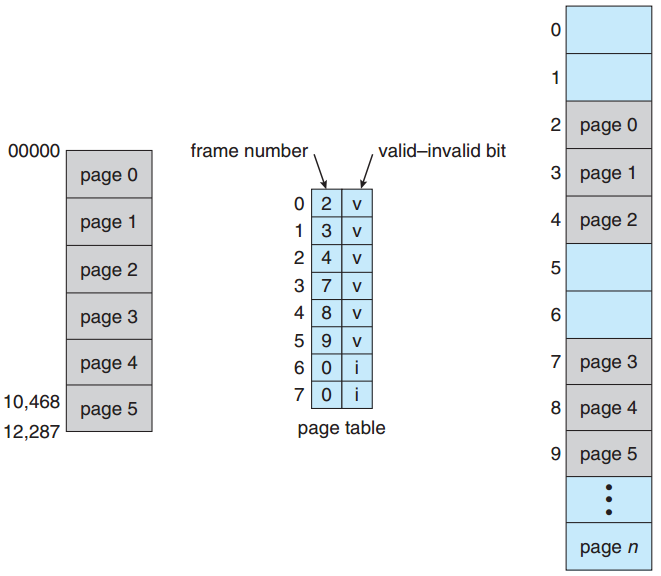
\includegraphics[scale=0.6]{img/paginacion_proteccion.png}
	\caption{Bit valido-invalido en una tabla de paginas}
\end{figure}

\subsection*{Segmentación}
La protección de memoria se logra con bits de protección asociados a cada marco. Estos bits normalmente se mantienen en la tabla de paginas.

Un bit podría indicar si una pagina es de lectura-escritura o solo lectura. Cuando se este calculando la dirección física, los bits de protección pueden ser revisados para verificar que no se hacen escrituras a una pagina de solo lectura. Esto puede extenderse para lograr un mayor nivel de protección, ya se a con hardware, o tener bits separados para cada tipo de acceso. Cualquier intento ilegal (por ejemplo, escritura en una pagina de solo lectura) causara un trap de hardware al sistema operativo.

Generalmente se asocia un bit adicional a cada entrada de la tabla de paginas, un bit válido-inválido. Cuando el bit esta en valido, la pagina asociada se encuentre en el espacio de direcciones lógicas del proceso y entonces es una pagina legal o valida. Si el bit esta en invalido, la pagina no se encuentre en el espacio de direcciones lógicas del proceso. Las direcciones ilegales se capturan utilizando este bit. El sistema operativo configura este bit para cada pagina para permitir o prohibir el acceso a dicha pagina.

\begin{figure}[H]
	\centering
	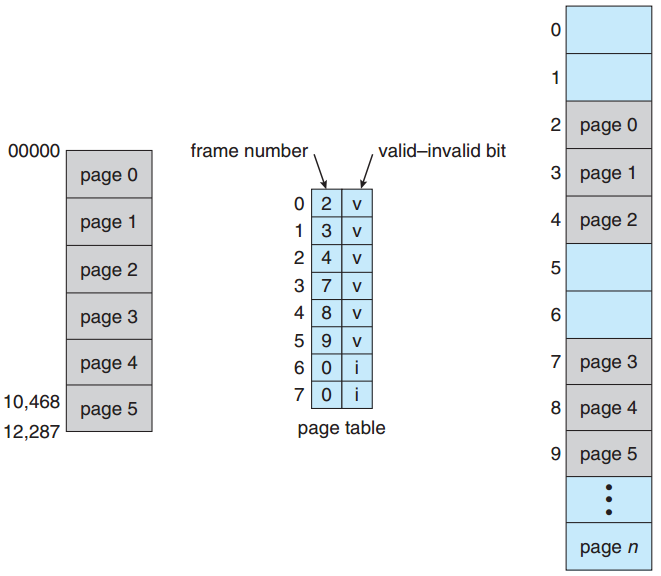
\includegraphics[scale=0.6]{img/paginacion_proteccion.png}
	\caption{Bit valido-invalido en una tabla de paginas}
\end{figure}
%-------------------------------------------------------%
%--% Bibliografia %-------%
%\newpage
%\nocite{*}
%\bibliographystyle{unsrt}
%\bibliography{bibliography}
%--------------------------%
\end{document}
